\chapter{Implementacija i korisničko sučelje}
		
		
		\section{Korištene tehnologije i alati}
		
		
			Komunikacija u timu ostvarena je pomoću aplikacija WhatsApp i Discord. Za upravljanje i verzioniranje izvornog koda korišten je Git te udaljeni repozitorij na web platformi GitLab.
			\vspace{3mm}
Za razvoj backenda kokrištena su razvojna okruženja (IDE) Eclipe i IntelliJ Idea, a za razvoj frontenda Visual Studio Code. Rad sa bazom podataka ostvaren je pomoću sustava PostgreSQL i pgAdmin. Aplikacija je napisana u programskim jezicima Java i JavaScript.
\vspace{3mm}
Backend aplikacije izrađen je u radnom okviru Spring Boot, koji sadrži brojne biblioteke za rad sa bazom podataka, izradu web aplikacije i sigurnost pri slanju HTTP zahtjeva. Za frontend je korištena biblioteka React koja se koristi za izgradnju korisničkih sučelja.
Aplikacija je hostana na cloud platformi Heroku. \\


\url{https://www.whatsapp.com} \\
\url{https://discord.com} \\
\url{https://git-scm.com} \\
\url{https://about.gitlab.com} \\
\url{https://www.eclipse.org/ide} \\
\url{https://www.jetbrains.com/idea} \\
\url{https://code.visualstudio.com} \\
\url{https://www.postgresql.org} \\
\url{https://www.java.com} \\
\url{https://www.javascript.com} \\
\url{https://spring.io} \\
\url{https://reactjs.org} \\
\url{https://www.heroku.com} \\
		
			\eject 
		
	
		\section{Ispitivanje programskog rješenja}
			
			Provedeno je automatizirano ispitivanje programskog rješenja. Testiranje komponenti sustava izvedeno je pomoću JUnit testova, a ispitivanje ponašanja sustava pomoću alata Selenium IDE.
	
			
			\subsection{Ispitivanje komponenti}
			Proveli smo 7 JUnit testova koji testiraju razrede i metode u aplikaciji.
			\vspace{3mm}
			
			\textbf{Ispitni slučaj 1: Prvi test testira registraciju novog usera u aplikaciji. }	
			
			\begin{figure}[H]
				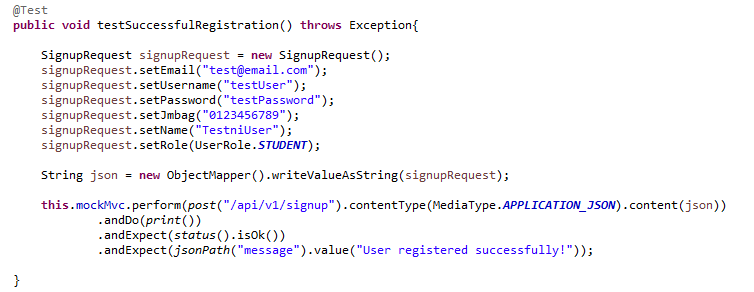
\includegraphics[scale=0.9]{slike/test1.PNG} %veličina slike u odnosu na originalnu datoteku i pozicija slike
				\centering
				\label{fig:test1}
			\end{figure}
			
			\textbf{Ispitni slučaj 2 i 3: Sljedeća dva testa testiraju hoće li se dogoditi iznimka u slučaju ako pokušamo 
registrirati novog korisnika u sustav ukoliko već postoji korisnik s istim usernameom ili se email 
već koristi.
}	
			
			\begin{figure}[H]
				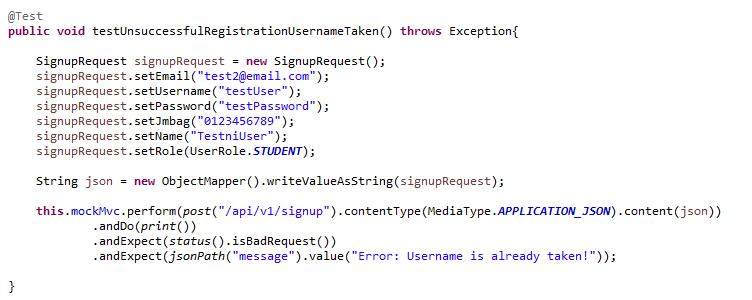
\includegraphics[scale=0.9]{slike/test2.PNG} %veličina slike u odnosu na originalnu datoteku i pozicija slike
				\centering
				\label{fig:test2}
			\end{figure}
			
			\begin{figure}[H]
				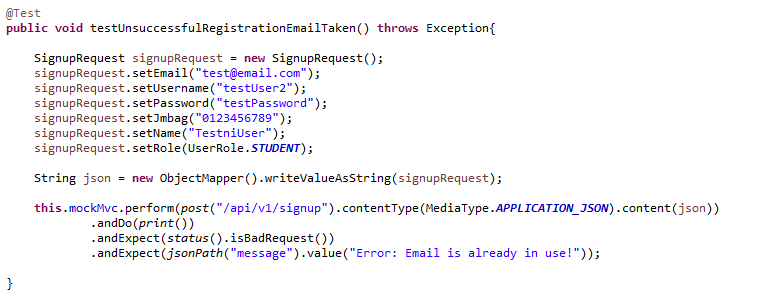
\includegraphics[scale=0.9]{slike/test3.PNG} %veličina slike u odnosu na originalnu datoteku i pozicija slike
				\centering
				\label{fig:test3}
			\end{figure}
			
			\textbf{Ispitni slučaj 4: Test 4 provjerava api koji vraća podatke o trenutačno logiranom korisniku.  }	
			
			\begin{figure}[H]
				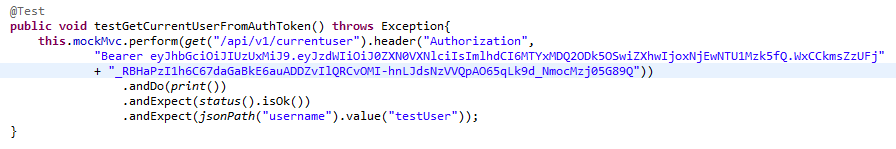
\includegraphics[scale=0.9]{slike/test4.PNG} %veličina slike u odnosu na originalnu datoteku i pozicija slike
				\centering
				\label{fig:test4}
			\end{figure}
			
			\textbf{Ispitni slučaj 5:Test 5 provjerava baca li se odgovarajuća iznimka kada se pokuša koristiti api za 
provjeru podataka o trenutačno logiranom korisniku, a odgovarajući JWT token nije bio poslan.}	
			
			\begin{figure}[H]
				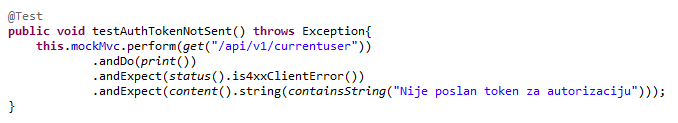
\includegraphics[scale=0.9]{slike/test5.PNG} %veličina slike u odnosu na originalnu datoteku i pozicija slike
				\centering
				\label{fig:test5}
			\end{figure}
			
			\textbf{Ispitni slučaj 6: Test 6 provodi provjeru logiranja u sustav. Ukoliko se korisnik uspješno ulogira, test prolazi.
}	
			
			\begin{figure}[H]
				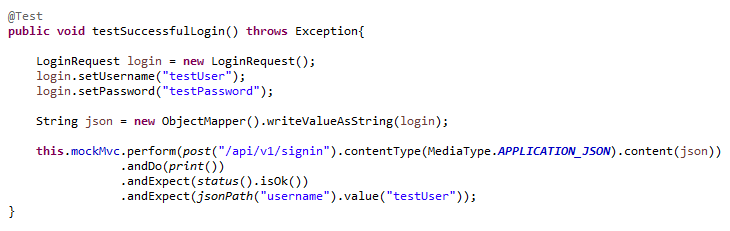
\includegraphics[scale=0.9]{slike/test6.PNG} %veličina slike u odnosu na originalnu datoteku i pozicija slike
				\centering
				\label{fig:test6}
			\end{figure}
			
			\textbf{Ispitni slučaj 7: Test 7 provjera što se će se dogoditi u slučaju neispravnih korisničkih podataka za login. 
Očekivano ponašanje je error kod 400 uz poruku "Bad credentials".
}	
			
			\begin{figure}[H]
				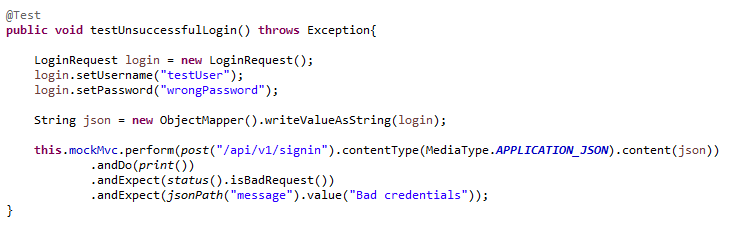
\includegraphics[scale=0.9]{slike/test7.PNG} %veličina slike u odnosu na originalnu datoteku i pozicija slike
				\centering
				\label{fig:test7}
			\end{figure}
			
			
			
			\subsection{Ispitivanje sustava}
			
			 Ispitivanje sustava provedeno je dodatkom za preglednik Selenium IDE. Testirani su slučajevi registracije, prijave korisnika, objave oglasa i oznake oglasa da se više ne prikazuje.
			 
			 \textbf{Ispitni slučaj 1:Registracija korisnika
}	
Testirana je registracija korisnika s jedinstvenim podatcima te je očekivani rezultat uspješna registracija.
			
			\begin{figure}[H]
				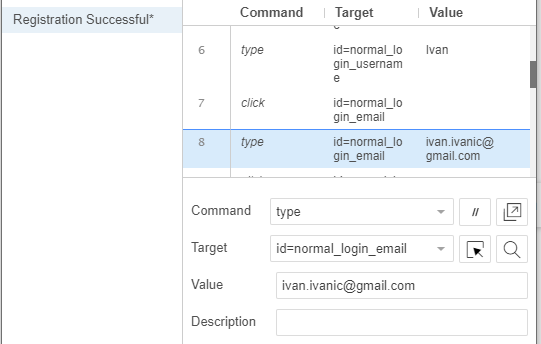
\includegraphics[scale=0.6]{slike/test8.PNG} %veličina slike u odnosu na originalnu datoteku i pozicija slike
				\centering
				\label{fig:test8}
			\end{figure}
			\begin{figure}[H]
				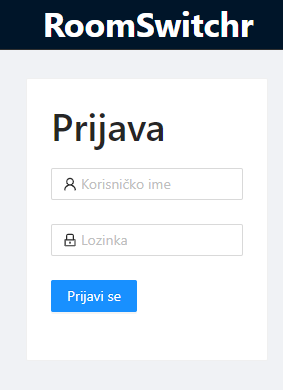
\includegraphics[scale=0.6]{slike/test8pom.PNG} %veličina slike u odnosu na originalnu datoteku i pozicija slike
				\centering
				\label{fig:test8pom}
			\end{figure}
			
			\textbf{Ispitni slučaj 2: Prijava nepostojećeg korisnika}	
			Testirana je prijava korisnika s nepostojećim korisničkim imenom te je očekivani rezultat odbijanje prijave i ispis poruke u grešci.
			
			\begin{figure}[H]
				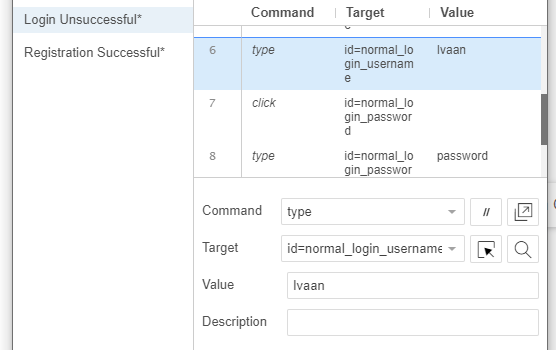
\includegraphics[scale=0.6]{slike/test9.PNG} %veličina slike u odnosu na originalnu datoteku i pozicija slike
				\centering
				\label{fig:test9}
			\end{figure}
			\begin{figure}[H]
				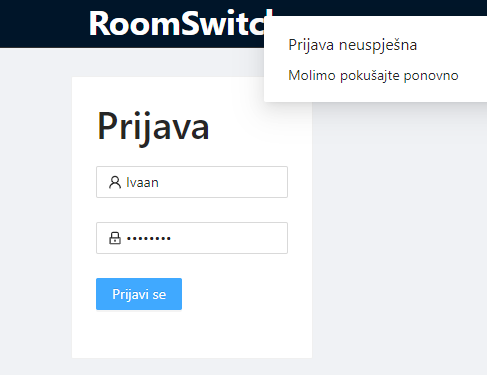
\includegraphics[scale=0.6]{slike/test9pom.PNG} %veličina slike u odnosu na originalnu datoteku i pozicija slike
				\centering
				\label{fig:test9pom}
			\end{figure}
			
			\textbf{Ispitni slučaj 3: Predaja oglasa}
			Testirana je predaja oglasa korisnika koji već ima aktivni oglas. Očekivani rezultat je stvaranje novog aktivnog oglasa, a prethodni aktivni oglas postaje neaktivan.	
			
			\begin{figure}[H]
				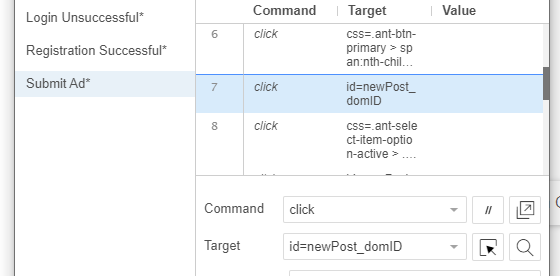
\includegraphics[scale=0.6]{slike/test10.PNG} %veličina slike u odnosu na originalnu datoteku i pozicija slike
				\centering
				\label{fig:test10}
			\end{figure}
			\begin{figure}[H]
				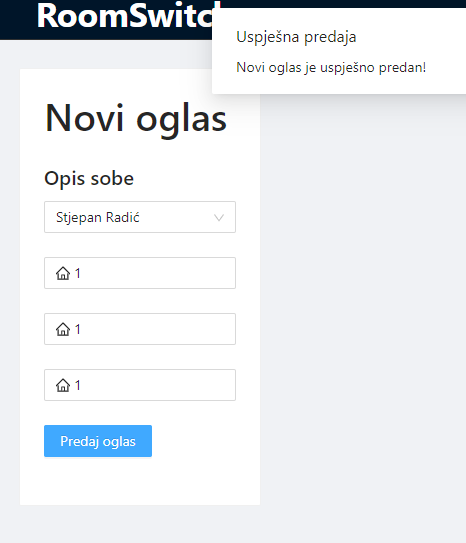
\includegraphics[scale=0.6]{slike/test10pom.PNG} %veličina slike u odnosu na originalnu datoteku i pozicija slike
				\centering
				\label{fig:test10pom}
			\end{figure}
			\begin{figure}[H]
				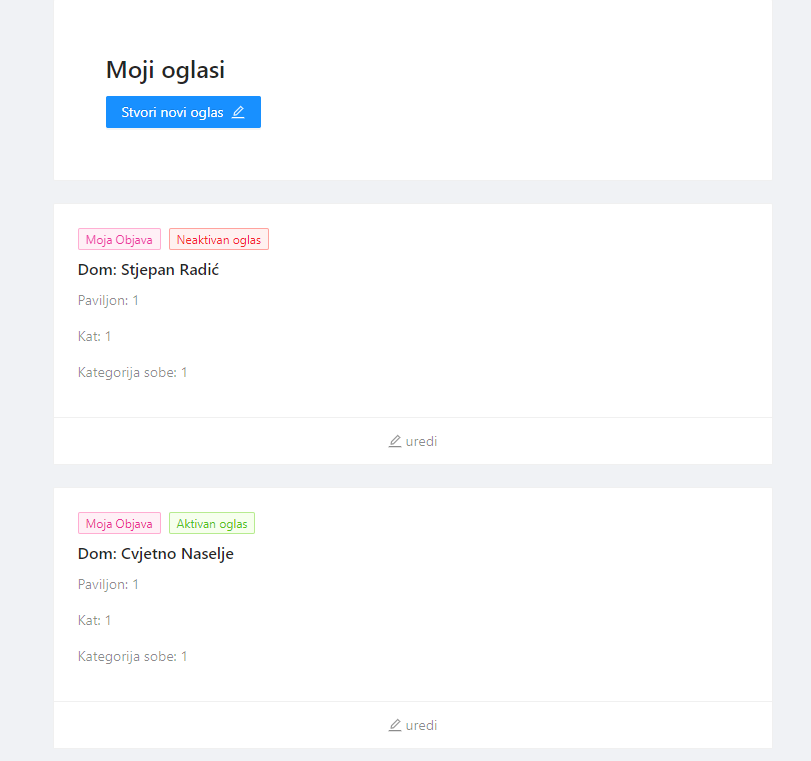
\includegraphics[scale=0.6]{slike/test10pompom.PNG} %veličina slike u odnosu na originalnu datoteku i pozicija slike
				\centering
				\label{fig:test10pom}
			\end{figure}
			
			\textbf{Ispitni slučaj 4: Ne prikazuj više ovaj oglas}	
			Testirano je označavanje oglasa da se više ne prikazuje te je očekivani rezultat početna stranica na kojoj nema označenog oglasa.
			
			\begin{figure}[H]
				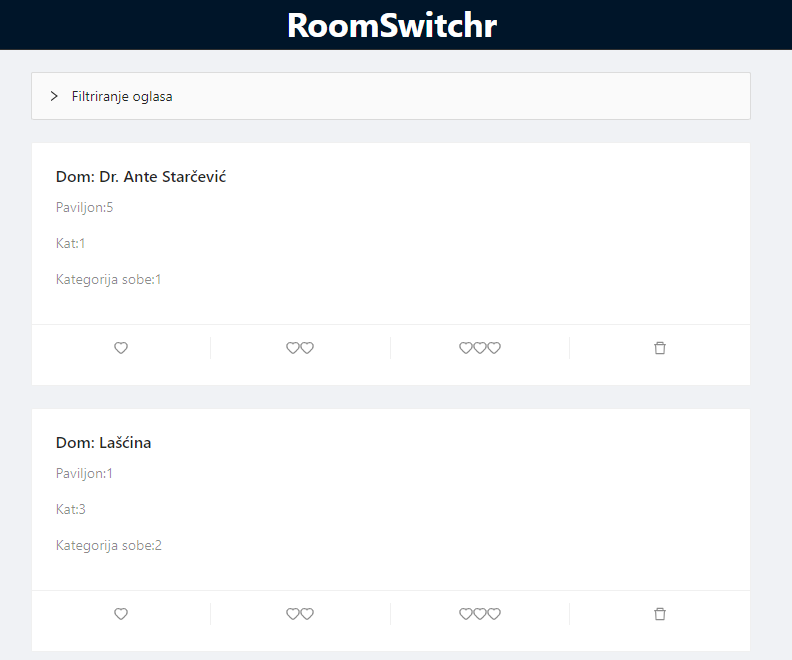
\includegraphics[scale=0.6]{slike/test11.PNG} %veličina slike u odnosu na originalnu datoteku i pozicija slike
				\centering
				\label{fig:test11}
			\end{figure}
			\begin{figure}[H]
				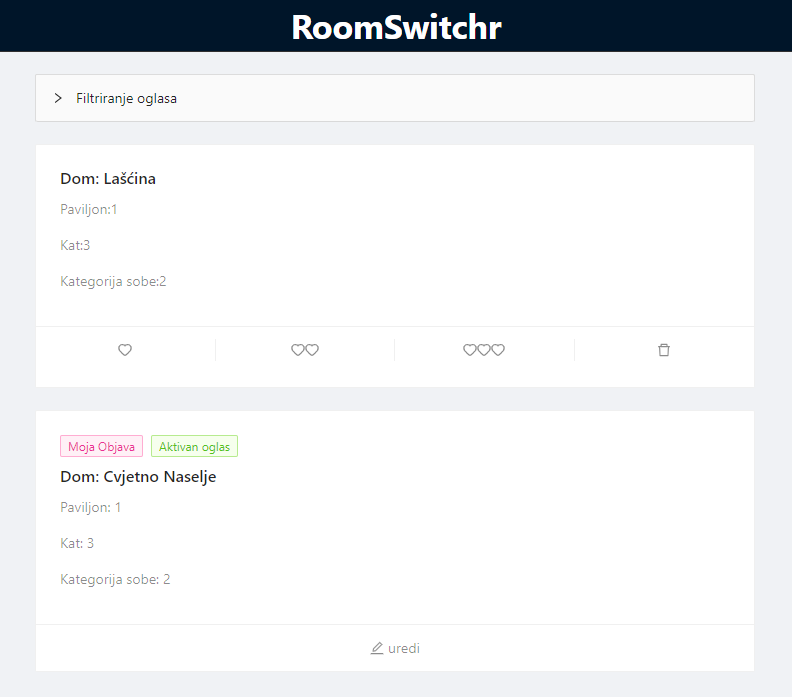
\includegraphics[scale=0.6]{slike/test11pom.PNG} %veličina slike u odnosu na originalnu datoteku i pozicija slike
				\centering
				\label{fig:test11pom}
			\end{figure}
			
			\eject 
		
		
		\section{Dijagram razmještaja}
			
			Dijagrami razmjestaja opisuju topologiju sklopovlja i programsku potporu koja se koristi u implementaciji sustava u njegovom radnom okruzenju. Na poslu žiteljskom
računalu se nalaze web poslužitelj i poslužitelj baze podataka. Klijenti koriste web preglednik kako bi pristupili web aplikaciji. Sustav je baziran na arhitekturi ”klijent – posluzitelj”, a komunikacija između računala korisnika (student ili djelatnik studentskog centra) i poslužitelja odvija se preko HTTP veze.
		
		\begin{figure}[H]
				\includegraphics[scale=0.5]{slike/dijag_razmještaja.PNG} %veličina slike u odnosu na originalnu datoteku i pozicija slike
				\centering
				\caption{Dijagram razmještaja}
				\label{fig:java}
			\end{figure}
			
			\eject
		
		\section{Upute za puštanje u pogon}

Potrebno je preuzeti PostgreSQL bazu podataka. Nakon toga potrebno je provesti standardnu instalaciju 
te se prijaviti s korisničkim imenom „postgres“ i lozinkom „bazepodataka“. 
Nakon instalacije, potrebno je pokrenuti pgAdmin i konfigurirati prvu konekciju na bazu. Potrebno je 
prijaviti se s istim korisničkim imenom i lozinkom kao i prilikom instalacije. U bazi podataka bi već 
trebala postojati tablica „postgres“. 
Server baze mora biti pokrenut. U daljnjim uputama opisan je način podizanja baze.
\vspace{3mm}

Kako bi se aplikacija pokrenula potrebno je instalirati podršku za bazu podataka, podršku za 
prevođenje i pokretnaje aplikacija napisanih u programskom jeziku Java te podršku za 
prevođenje i pokretnaje aplikacija napisanih u programskom jeziku JavaScript.
\vspace{3mm}

Prilikom instalacije podrške za bazu podataka potrebno je preuzeti aplikaciju pgAdmin s poveznice
\url{https://www.pgadmin.org/download/}. Nakon preuzimanja, potrebno je provesti standardnu instalaciju 
te se prijaviti s korisničkim imenom „postgres“ i lozinkom „bazepodataka“.
Nakon instalacije, potrebno je pokrenuti pgAdmin i konfigurirati prvu konekciju na bazu. Potrebno je 
prijaviti se s istim korisničkim imenom i lozinkom kao i prilikom instalacije. U bazi podataka bi već 
trebala postojati tablica „postgres“. Server baze tijekom korištenja aplikacije mora biti pokrenut.
Na računalu je također potrebno instalirati podršku za programski jezik Java (\url{http://jdk.java.net/15}).
Također kako bi se mogli pokretati programi napisani u JavaScriptu potrebno je instalirati Node.js 
(\url{https://nodejs.org/en/download}). 
\vspace{3mm}
Osim podrški za pokretanje programa, potrebno je instalirati i razvojnu okolinu. Najjednostavnije je instalirati
IDE Intelij jer se u njemu mogu pokretati programi napisani i u jeziku Java i u jeziku JavaScript.
Projekt se može preuzeti s poveznice \url{https://gitlab.com/mariakatic/piccologrupa}.
Nakon uspješne isntalacije svega od navedenog, konačno se može pokrenuti aplikacija. 
Potrebno je instalirati npm pakete pokretanjem naredbe npm install. Frontend se pokreće naredbom npm start, a 
backend pritiskom tipke Run u razvojnom okruženju.
Nakon pokretanja programa, aplikacija se može pregledati u pregledniku na poveznici http://localhost:3000.
\vspace{3mm}
Na gore opisan način pokreće se aplikacija neovisno o tome je li deployana. Ova aplikacija hostana je na 
cloud platofrmi Heroku te se također može pronaći na linku \url{https://switchr.herokuapp.com}.
			
			
			\eject 